\documentclass{article}

% IMPORT PACKAGES
\usepackage{graphicx}
\graphicspath{{images/}}
\usepackage{blindtext}
\usepackage[T1]{fontenc}
\usepackage[latin9]{inputenc}
\usepackage[a4paper]{geometry}
\geometry{verbose,tmargin=2cm,bmargin=2cm,lmargin=1cm,rmargin=1cm}
\setlength{\parskip}{\smallskipamount}
\setlength{\parindent}{0pt}
\usepackage{array}
\usepackage{mathtools}
\usepackage{dsfont}
\usepackage{amsmath}
\usepackage{amssymb}
\usepackage{lmodern}
\usepackage{eqlist}
\usepackage{babel}
\usepackage{multicol}
\usepackage{stackengine}
\usepackage{xcolor}
\usepackage{listings}
% BLOCKS
\usepackage{beamerarticle}
\usepackage[most]{tcolorbox}
%	COMMON COLORS
\definecolor{_light_green}{rgb}{0.36, 0.84, 0.36}
\definecolor{_light_grey}{rgb}{0.90, 0.90, 0.90}
\definecolor{_white}{rgb}{1.0, 1.0, 1.0}
\definecolor{_blue}{rgb}{0.0, 0.0, 1.0}
\definecolor{_light_blue}{rgb}{0.7, 0.9, 1.0}
%	DEFINE BOXES
\newtcolorbox{_block}[1][]{
    colbacktitle=_light_grey,		% title background
    coltitle=black,					% title color
    titlerule=0pt,
    colback=white!50!_light_grey,	% body background
    boxrule=0.4pt,					% content-frame padding (or frame width)
    colframe=black!20!_light_grey,	% frame color
    left=0mm,						% content and title left padding
    arc=0.5pt,						% border-radius
    title={#1},
}
\newtcolorbox{_example}[1][]{
    colbacktitle=_light_green,
    coltitle=black,
    titlerule=0pt,
    colback=white!60!_light_green,
    boxrule=0pt,
    colframe=white,
    left=0mm,
    arc=0.5pt,
    title={#1},
}
\newtcolorbox{_note}[1][]{
    colbacktitle=_light_blue,
    coltitle=black,
    titlerule=0pt,
    colback=white!60!_light_blue,
    boxrule=0pt,
    colframe=white,
    left=0mm,
    arc=0.5pt,
    title={#1},
}
\newtcolorbox{_block_emph}[1][]{
    enhanced,
    frame hidden,
    borderline west={2.0pt}{0pt}{blue!60!white},
    opacityframe=0.0,
    colback=blue!4!white,
    left=2mm,
    arc=0.5pt,
    title={#1},
}
%   CUSTOM CODE LISTINGS
\newtcblisting{code}[2][]{
	colback=blue!5!white,
	colframe=red!75!black,
	opacityframe=0.0,
	coltitle=black,
	left=5pt,
	lefttitle=0pt,
	enhanced,
	listing only,
	title=\textbf{#2},
	arc=0.5pt,
	listing engine=minted,
	minted language={#1},
	minted style=colorful,
	minted options={
		fontfamily=\sfdefault,%\sserif
		fontsize=\scriptsize,
		breaklines,
		autogobble, %linenos, %numbersep=1mm,
		tabsize=4,
		escapeinside=||,mathescape=true,
	},
	overlay={
		\begin{tcbclipinterior}
			\fill[black!30!white] (frame.south west) 
			rectangle ([xshift=1mm]frame.north west);
		\end{tcbclipinterior}
	},
}

% below command to set inline code style doesn't work    :(
\lstset{language=C,keywordstyle={\bfseries \color{blue}}}

% \usepackage{subfiles}
% \subfile{}

% DOCUMENT

\begin{document}

% short title:
%   \part*{}
%   \part[]{}

\title{CS3237 Introduction to Internet of Things \\ Group 4 Report}
\author{Lai Yu Heem, Pinkl Constantin Maxime, Teo Chuan Kai, Wong Chee Hong, Thomm Leon Felix}
\maketitle

% changing sections enumeration style
% styles: \arabic{} \alph{} \Alph{} \roman{} \Roman{}
\renewcommand\thesection{\arabic{section}}
\renewcommand\thesubsection{\thesection.\alph{subsection}}

\newcommand\ISquaredC{$\text{I}^2\text{C}$}

\section{Abstract}

\textbf{???}

\section{Introduction}

\textbf{Tino}

\section{Solution Approach}

\subsection{Architecture overview}

\begin{multicols}{2}

Physically, the system consists of two components: the \textit{cloud} and the \textit{buoy(s)}, whereas a buoy can be further divided into \textit{WeMOS} and \textit{phone}. 

The WeMOS collects most of the data of interest (temperature, movement, water turbidity). It then sends collected records to the phone via WiFi, which extends it and does some timestamp modification.

The phone also serves as a gateway and forwards the records to the server running in the cloud.

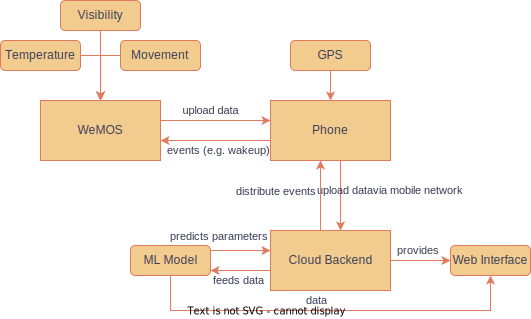
\includegraphics[width=9cm]{report/resources/architecture.png}

\end{multicols}

\subsection{Buoy Hardware}

\begin{multicols}{2}

The WeMOS collects most of the data. In particular, we collected

\begin{itemize}
    \item water temperature
    \item movement (accelerometer, gyroscope)
    \item water turbidity
\end{itemize}

For temperature, we used the tiny module from the set, sticking out of the buoy into the water. The water turbidity was implemented using an LED shining light through a section of water, and a photoresistor on the other side.

Temperature sensor and photoresistor were connected to the ADC, and accelerometer data was supplied from the MPU. ADC and MPU are both communicating with the WeMOS over \ISquaredC.

\includegraphics[width=9cm]{report/images/wiring.png}

\end{multicols}

\subsection{Phone applications}

\textbf{Tino}

\subsection{Server-side}

\textbf{Chuan Kai}

\subsection{ML model and application}

\textbf{Yu Heem}

\subsection{Front-End}

\textbf{Chuan Kai}

\section{Implementation Details}

\subsection{Turbidity sensor}

\textbf{Chee Hong}

\subsection{Waterproofing}

\textbf{Chee Hong}

\subsection{Power modes and sampling frequencies}

One of the most important bottlenecks is obviously power supply, because the buoy must run on battery. To increase lifetime, we had the following idea:

\begin{multicols}{2}

\begin{_block}[]
Employ two different power modes:
\begin{enumerate}
    \item \textbf{intense}: high frequency data collection ($f_H$)
    \item \textbf{chill}: low frequency data collection ($f_L$)
\end{enumerate}
\end{_block}

Mainly for simplicity- and demo-purposes we chose $f_H=1s$ and $f_L=10s$.

Using different data collection intensity modes suggests employing different power modes of the WeMOS. Unfortunately, because the data transfer between WeMOS and phone is WiFi-based, for the above frequencies it was not feasable to put the WeMOS in \textit{light sleep mode} as this kills the WiFi connection, and connecting to the hotspot was not too reliable.

Notice that \textit{deep sleep mode} is not useful because it puts the whole WeMOS to sleep, including \ISquaredC\ devices, and the MPU shouldn't be moving in order to calibrate.

In real application one would probably significantly increase the delay in chill mode.

\begin{code}[c]{WeMOS scheduler}
<-snip->
namespace scheduler {
    int last_fetch;
    bool intense = true;
    int last_time_intense_detected = 0;
    
    void init() { <-snip-> }
    void set_intense(){ <-snip-> }
    void set_chill(){ <-snip-> }
    int get_delay(){ <-snip-> }

    // return delay time until next fetch
    void wait() { <-snip-> }
    
    // update mode based on most recent measurements
    // if amplitudes exceed threshold, wake up
    void update(float g_force, float brightness){ <-snip-> }
}
\end{code}

\end{multicols}

\subsection{\ISquaredC\ Communication}

\begin{multicols}{2}

The communication between ADC, MPU, and WeMOS is based on \ISquaredC. We first tried to rely on well-engineered libraries for this, which didn't work out well initially - apparently there are subtle differences between the same components built by different manufacturers and we ran into tons of issues.

This caused us to write the code for the ADC ourselves (based on the Lab and the provided spec sheet), which worked well initially. However, after a while we again couldn't initialize any devices, as register assignments to multiplex the analog ports seemed to switch randomly sometimes. We eventually managed to get it working using the \lstinline{ADS1115_WE} library.

For the MPU we ended up using the \lstinline{MPU6500_WE} library, which is impressively feature-rich.

The combination of MPU, ADC, and \ISquaredC\ made reading from the sensors mostly reliable and comparably easy to debug.

\begin{code}[c]{ADC \ISquaredC}
#include <ADS1115_WE.h>
namespace adc {
    <-snip->
    float read(int channel) {
        float voltage = 0.0;
        ADS1115_MUX c;
        switch (channel) {
            case 0: c = ADS1115_COMP_0_GND; break;
            <-snip->
        }
        _adc->setCompareChannels(c);
        _adc->startSingleMeasurement();
        while(_adc->isBusy()){}
        return _adc->getResult_V() / 3.3;
    }
}
\end{code}

\end{multicols}

\subsection{Buoy-Server}

\textbf{Chuan Kai}

\subsection{Data collection}

\textbf{Tino}

\section{Experimental Evaluation}

\subsection{Model accuracy}

\textbf{Chuan Kai}

\subsection{Power consumption estimates}

\textbf{Leon}

\section{Challenges and Outlook}

\subsection{Phone reliance}

\textbf{Tino}

\subsection{Data bottleneck}

\textbf{Yu Heem}

\subsection{Statistical methods}

\textbf{Chee Hong}

\subsection{Other use-cases}

\textbf{???}

\subsection{...}

\end{document}